Bevor wir uns mit unendlichen Mengen befassen, sollten wir uns darüber im Klaren sein, dass unser ``gesunder Menschenverstand'' ein gefährlicher Begleiter auf diesem Weg sein kann. Um zu sehen, wie heikel die Vermischung von alltäglichen Konzepten mit der Vorstellung des Unendlichen sind, betrachten wir ein Hotel mit unendlich vielen Zimmern -- das sogenannte Hilbert Hotel.
\begin{example}[Hilbert's Hotel]
Hilbert's Hotel hat unendlich viele Zimmer, für jede natürliche Zahl eines.
\begin{center}
\begin{framed}
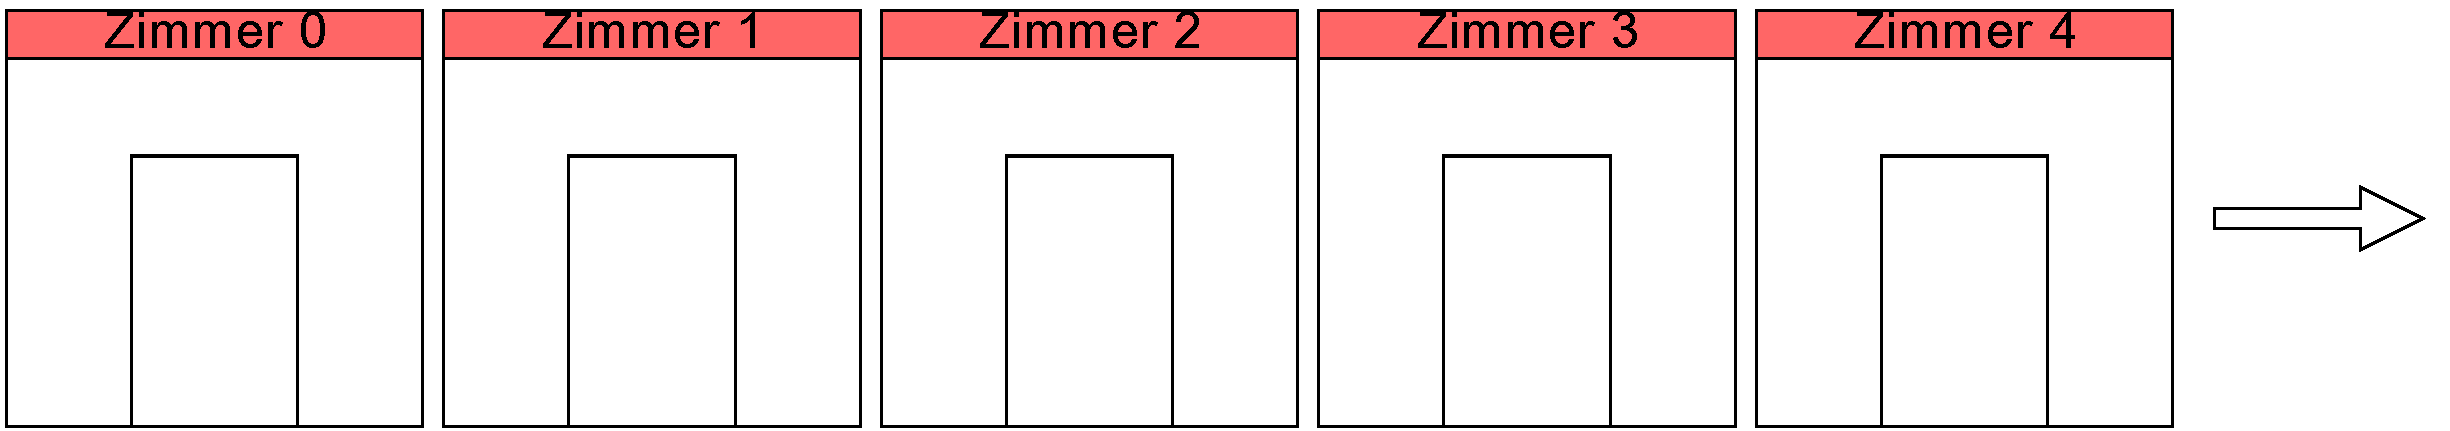
\includegraphics[width=0.9\textwidth]{figures/hilbertHotel}
%\caption*{Hilbert's Hotel}
\end{framed}
\end{center}
Im Rahmen eines Ferienjobs haben Sie eine Stelle als Concierge in Hilbert's Hotel angenommen\footnote{Sie verdienen schliesslich für jedes Zimmer einen Franken pro Arbeitstag.}. An Ihrem ersten Arbeitstag haben Sie die Nachtschicht. Herr Hilbert, der Hotelbesitzer, hat sich bereits zu seinem wohlverdienten Feierabend verabschiedet, als unvermittelt ein älterer Herr (ä.H.) die Lobby betritt.
\begin{itemize}
\item[ä.H.:] Ich bräuchte ein Zimmer in Ihrem Hotel.
\item[Sie:] Es tut mir leid, wir sind voll belegt. Ich könnte Ihnen aber das Hotel ``Cantors Paradise'' empfehlen. Es ist hier ganz in der Nähe, hier steht die Adresse.

\textit{Sie überreichen dem ä.H. eine Visitenkarte vom ``Cantors Paradise''.}
\item[ä.H.:] Mein lieber Concierge, laut Werbebroschüre hat Ihr Hotel unendlich viele Zimmer. Wie soll denn das bitte ausgebucht sein?
\item[Sie:] Na ja, wir haben im Moment unendlich viele Gäste -- in jedem Zimmer einen.
\item[ä.H.:] Das lass ich mal Ihr Problem sein! Mir genügt es, dass hier schwarz auf weiss steht, dass man angeblich keine Reservation zu tätigen braucht, um in diesem Hotel unterzukommen. Zudem werben Sie, mit Bezugnahme auf die Unendlichkeit Ihres Hotels, damit, dass jedem Gast und zu jeder Zeit ein Zimmer garantiert werden kann!

\textit{Der ä.H. kramt genervt seine Werbebroschüre hervor und zeigt sichtlich irritiert auf die entsprechende Seite.}
\item[Sie:] Hmm, ich werde sehen, ob sich da vielleicht doch was machen lässt. Bitte gedulden Sie sich einen Moment.

\textit{Der ä.H. lässt sich auf die grosse Couch fallen, die in der Eingangshalle steht. Sie, nicht ohne ein ziemlich ungutes Gefühl dabei zu haben, wählen Hilberts private Telefonnummer.}
\item[Hi.:] Hilbert am Apparat.
\item[Sie:] Entschuldigen Sie die späte Störung Herr Hilbert. Es ist mir unendlich unangenehm, aber ich habe hier im Hotel ein Problem.
\item[Hi.] Worum geht es denn?
\item[Sie:] Ich habe einen Gast, der trotz Vollbelegung auf ein Zimmer besteht. Und er kann sich erst noch auf unsere eigene Broschüre stützen, in der ja steht, dass wir nie ausgebucht seien, selbst dann nicht, wenn wir mal voll sein sollten!
\item[Hi.:] Ach ja, ich hatte vergessen Sie darauf aufmerksam zu machen. Alle unsere Gäste haben sich beim Bezug ihres Zimmers, {\tiny im Kleingedruckten}, damit einverstanden erklärt, dass wir sie im Notfall ein einziges Mal umplatzieren können. Nutzen Sie diese Klausel um unserem Gast ein Zimmer freizumachen. Noch etwas, machen Sie das Zimmer so frei, dass sie weitere Gäste, die vielleicht später noch kommen, ebenfalls noch unterbringen könnten und bedenken Sie stets, dass jeder Gast höchstens einmal umplatziert werden darf.

\textit{Sie beenden das Gespräch und wenden sich dem ungeduldig wartenden ä.H. zu.}
\item[Sie:] Sehr geehrter Herr, wir haben ein Zimmer für Sie gefunden, sie müssen sich bloss zwei Minuten gedulden, dann können Sie einziehen.
\item[ä.H.:] Sehen Sie, geht doch!
\end{itemize}
Wie bringen Sie den ä.H. unter? Bringen Sie weitere Gäste unter? Was machen Sie, wenn ein voller Limesbus (ein Bus mit unendlich vielen Sitzplätzen) ankommt? Wie lange dauert es bis der ganze Limesbus untergebracht wird?
\end{example}

\begin{example}
    Können wir mit Sicherheit sagen, dass mindestens zwei Menschen die selbe Anzahl an Haaren am Körper haben?
    \tcblower
    Wir teilen die Menge aller Menschen wie folgt in Gruppen $G_0,G_1,\dots$ ein
    \begin{align*}
    G_i=\text{ Alle Menschen, die genau $i$ viele Haare am Körper haben.}
    \end{align*}
    Weil jeder Mensch definitiv weniger als $10$ Mio. Haare besitzt (vgl. \url{https://bionumbers.hms.harvard.edu/bionumber.aspx?id=101509}) und weil definitiv mehr als $10$ Mio. Menschen existieren, können wir gemäss dem Schubfachprinzip darauf schliessen, dass es mindestens eine Gruppe mit mehreren Menschen darin gibt (also Menschen mit exakt der gleichen Anzahl an Haaren).
\end{example}

\begin{example}
    Die Funktion
    \begin{align*}
        &f :\N\to\N\\
        &f(x) =
            \begin{cases}
                \frac{x}{2}&\text{falls $x$ gerade}\\
                3x+1&\text{sonst}
            \end{cases}
    \end{align*}
    Ist surjektiv aber nicht injektiv. Wenn Sie die Funktion so wie im vorhergehenden Beweis im Schritt von $F_1$ zu $B_{\N,A}$ anpassen, welchen Funktionswert erhalten Sie dann für die Eingabe $8$?
    \tcblower
    $f(9)=28$
\end{example}


\begin{example}
Die Menge aller geraden natürlichen Zahlen ist abzählbar.
\begin{proof}{Abzählbarkeit zeigen durch Surjektive Abbildung}
Ist $G$ die Menge der geraden Zahlen, dann folgt die Behauptung aus der Tatsache, dass die Funktion
\[
F:\N\to G \phantom{abstand}\text{ mit }\phantom{abstand}F(n)=2n
\]
jede gerade natürliche Zahl trifft (und somit surjektiv ist).
\end{proof}
Dass die Menge der geraden natürlichen Zahlen auch anschaulich abzählbar ist, kann man sich etwa mit folgender Auflistung vergegenwärtigen:
\begin{center}
\begin{tabular}{c|c}
$\N$ & $G$\\
\hline
$0$ & $0$\\
$1$ & $2$\\
$2$ & $4$\\
$\vdots$ & $\vdots$
\end{tabular}
\end{center}
\end{example}

\begin{example}
Die Menge $\Z$ der ganzen Zahlen ist abzählbar.
\begin{proof}{Abzählbarkeit zeigen durch Surjektive Abbildung}
Wir müssen eine Funktion $F:\N\to\Z$ angeben, die jedes Element von $\Z$ trifft. Dies gelingt uns wie folgt:
\begin{align*}
F(n)=\begin{cases}
-\frac{n}{2} &\text{falls $n$ gerade}\\
\frac{n+1}{2}&\text{falls $n$ ungerade. }
\end{cases}
\end{align*}
\end{proof}
Anschaulich ergibt sich durch die Funktion $F$ folgende Auflistung der ganzen Zahlen:
\begin{center}
\begin{tabular}{c|c}
$\N$ & $\Z$\\
\hline
$0$ & $0$\\
$1$ & $1$\\
$2$ & $-1$\\
$3$ & $2$\\
$4$ & $-2$\\
$5$ & $3$\\
$\vdots$ & $\vdots$
\end{tabular}
\end{center}
\end{example}

\begin{example}
Die Menge aller \textit{endlichen} Sequenzen der Buchstaben $a,b$ ist abzählbar unendlich. Eine mögliche Auflistung der endlichen Sequenzen ist etwa durch
\begin{center}
\begin{tabular}{c|c}
$\N$ & $X$\\
\hline
$0$ & $a$\\
$1$ & $b$\\
$2$ & $aa$\\
$3$&$ab$\\
$4$&$ba$\\
$5$&$bb$\\
$6$&$aaa$\\
$7$ & $aab$\\
$8$ & $aba$\\
$9$ & $abb$\\
$\vdots$ & $\vdots$
\end{tabular}
\end{center}
gegeben.
\end{example}
\begin{example}
Die Menge aller Java, C, C\#, C++,Fortran\dots Programme ist abzählbar.
\tcblower
Wenn jedes Programm mit seinem Bytecode identifiziert wird, dann entspricht jedes Programm einer endlichen $0,1$-Folge. Diese können, gleich wie endliche $a,b$-Sequenzen, abgezählt werden.
\end{example}

\begin{example}
Ist die Menge aller endlichen Teilmengen von $\N$ abzählbar? Begründen Sie Ihre Antwort.
\tcblower
Wir können jede endliche Menge von natürlichen Zahlen mittels ihrer charakteristischen Funktion (vgl. Vorlesung) mit einer endlichen Binärsequenz identifizieren. Durch das Hinzufügen einer führenden $1$ zu jeder endlichen Binärsequenz entspricht jede dieser Sequenzen einer natürlichen Zahl in Binärdarstellung. Daraus folgt die Behauptung.
\end{example}

\begin{example}
Zeigen Sie, dass die Menge
\[
U=\{1,11,111,1111,\dots \}
\]
aller endlichen Sequenzen von Einsen abzählbar ist. Ist die Menge aller (abzählbar) unendlichen Sequenzen von Einsen auch abzählbar?
\tcblower
Wir müssen zeigen, dass eine surjektive Abbildung $F:\N\to \{1,11,\dots\}$ existiert. Da dies z.B. für die Funktion
	\begin{align*}
	F(n)=\underbrace{11\dots 1}_{n\text{ viele}}
	\end{align*}
	erfüllt ist, gilt die Behauptung. Die Menge aller (abzählbar) unendlichen $1$-Sequenzen besteht aus nur einem Element und ist somit natürlich abzählbar.
\end{example}